\section{opgave c}

\begin{figure}[h]
    \centering
    \caption{$\psi$ at $Re = 16$ for different grid sizes}\label{fig:grids}
    \centerline{
    \begin{subfigure}[b]{0.6\textwidth}
        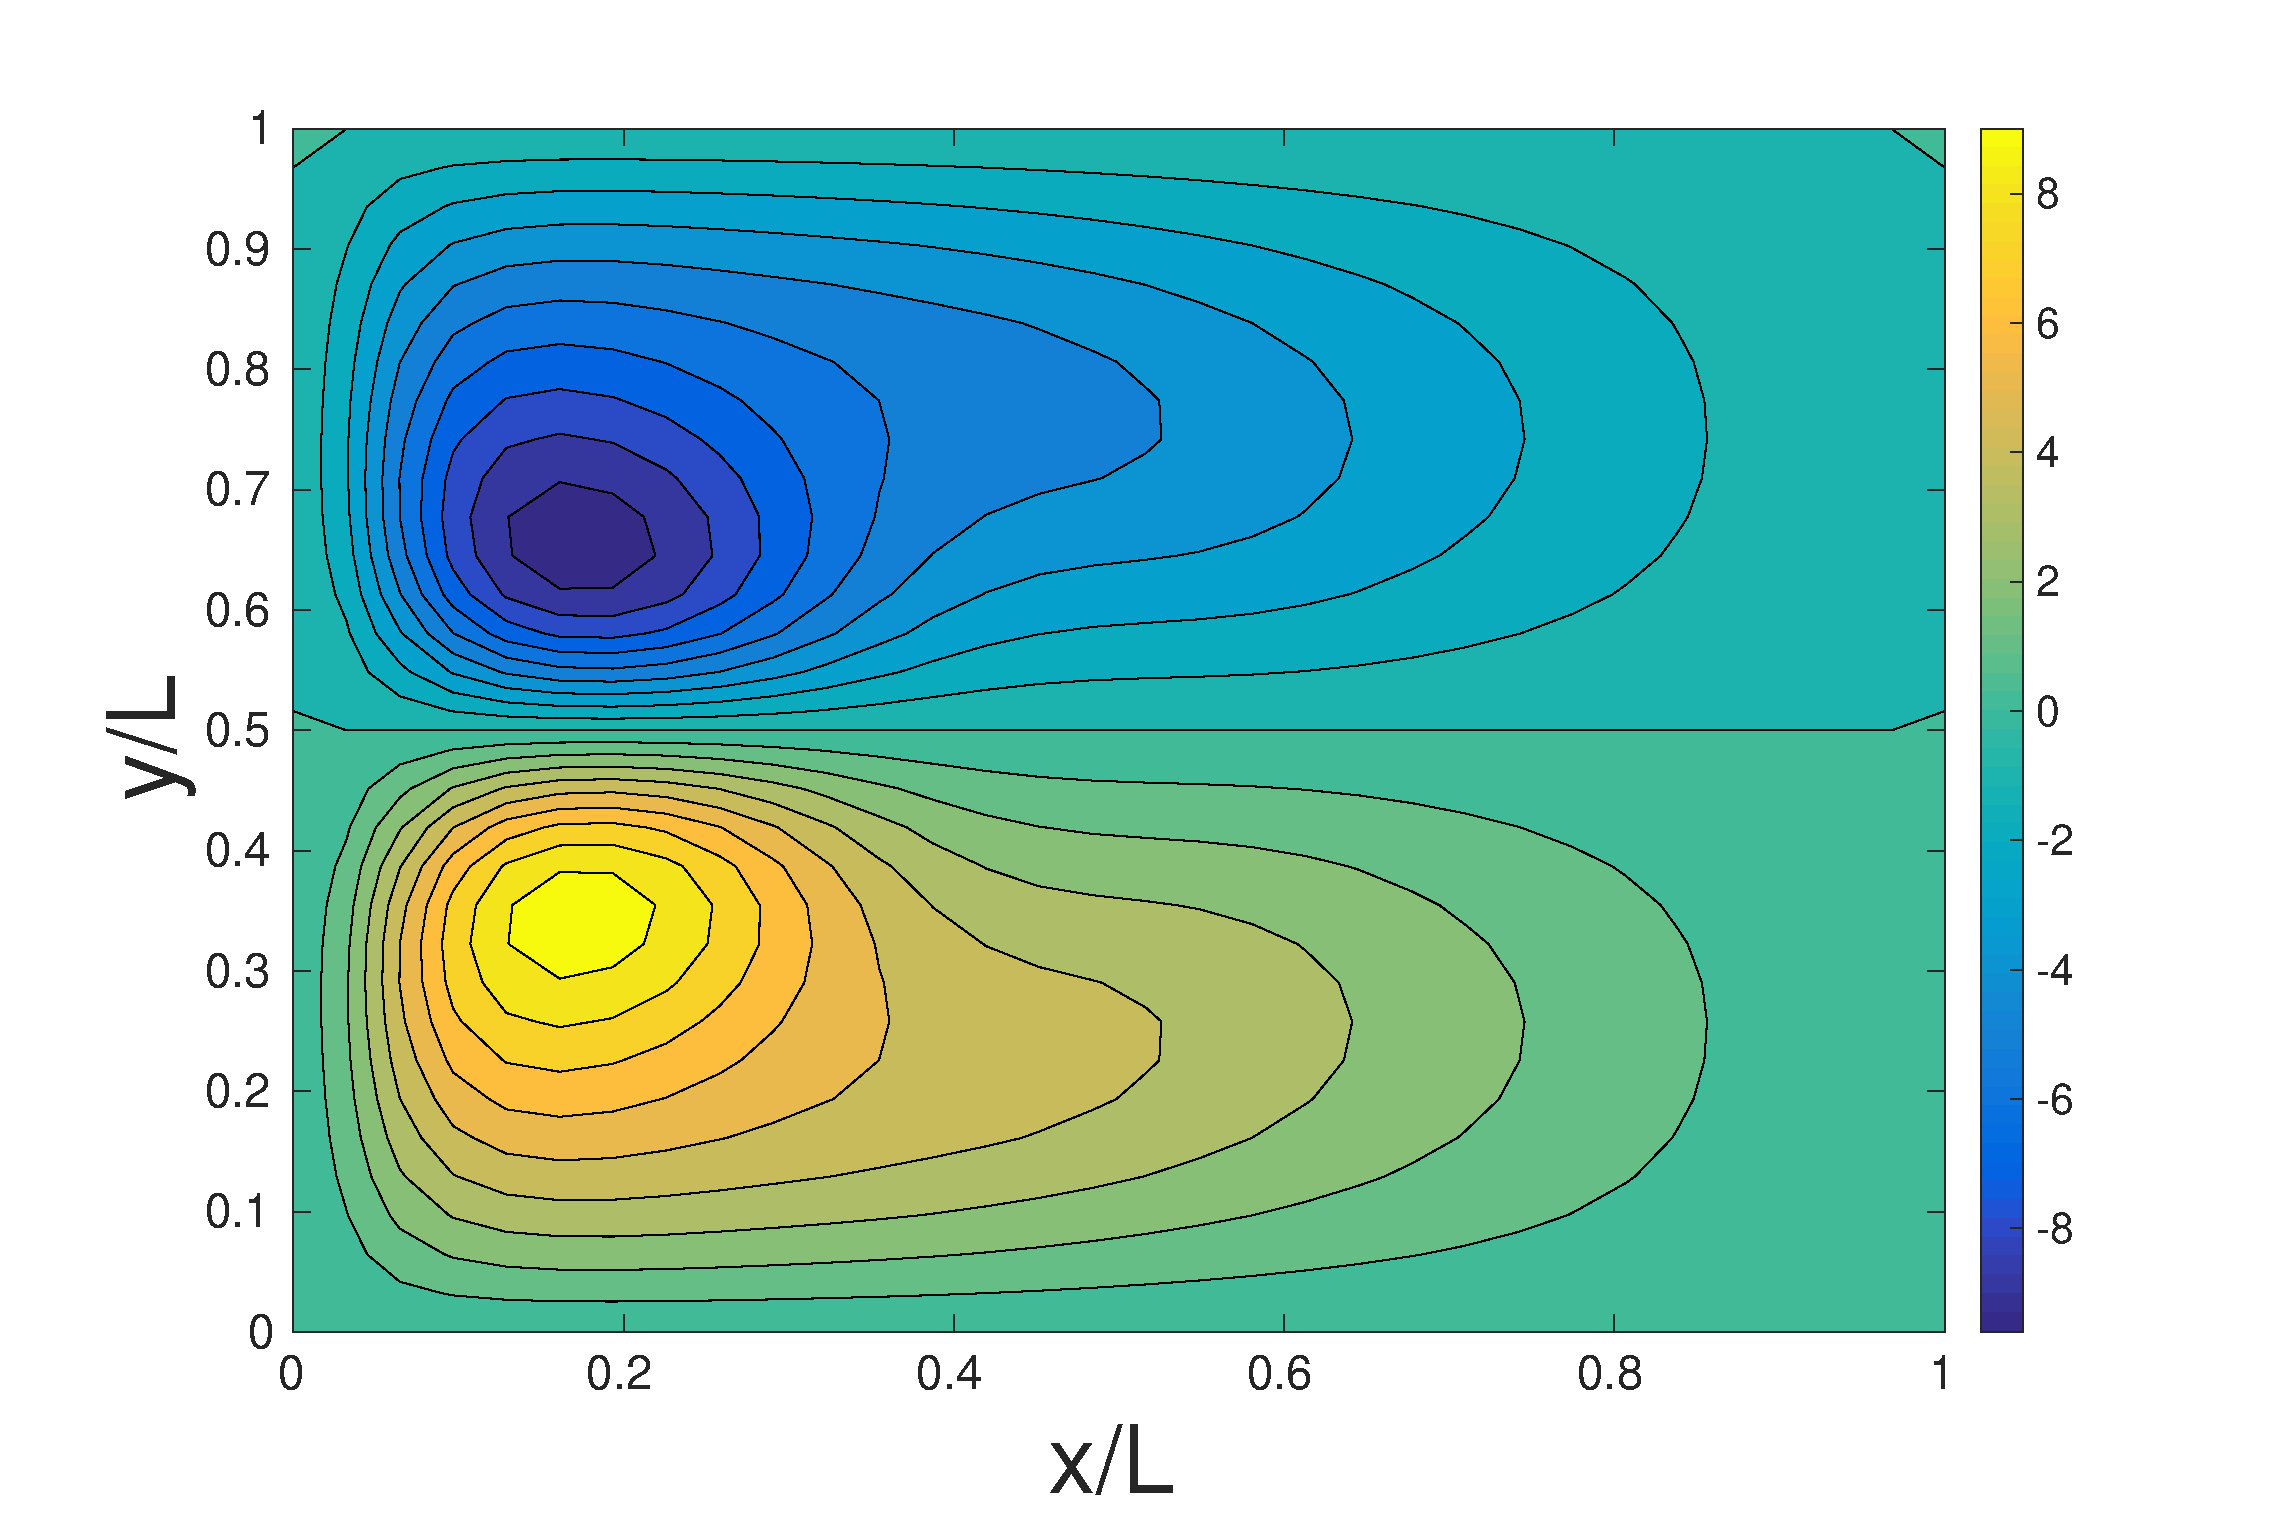
\includegraphics[width=\textwidth]{images/grid32.eps}
        \caption{$32\times 32$}
        \label{fig:nm32}
    \end{subfigure}
    ~
    \begin{subfigure}[b]{0.6\textwidth}
        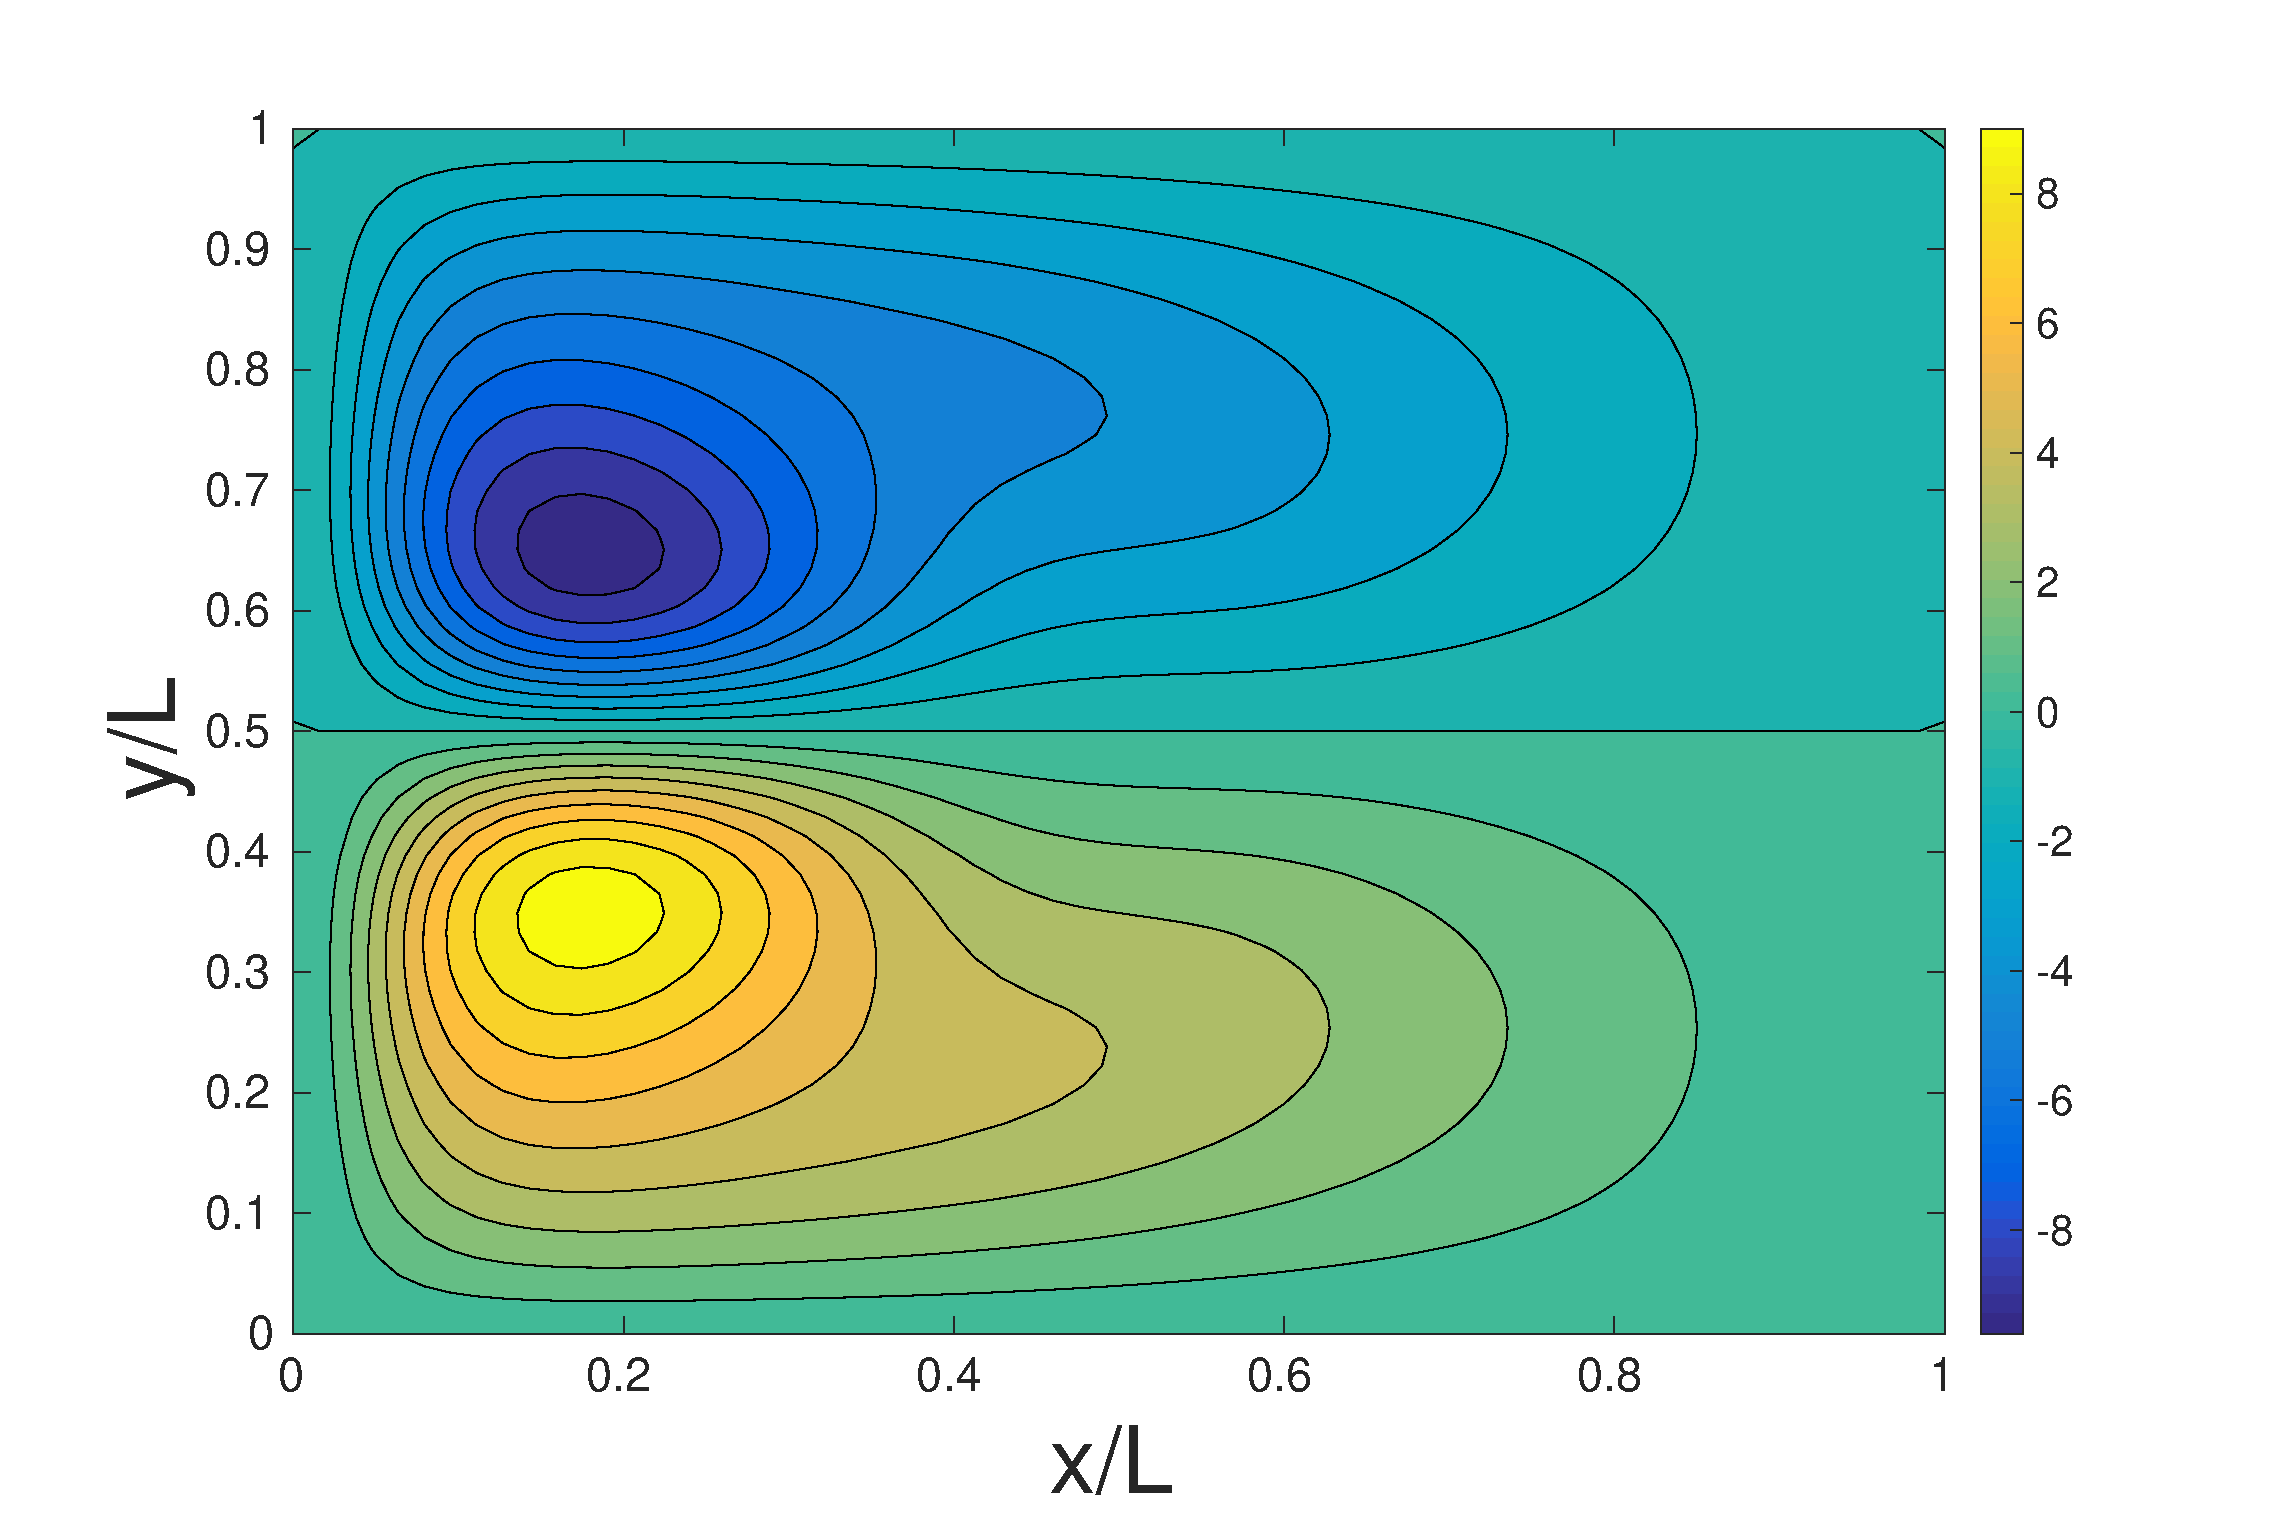
\includegraphics[width=\textwidth]{images/grid64.eps}
        \caption{$64\times 64$}
        \label{fig:nm64}
    \end{subfigure}
    }
    
    \begin{subfigure}[b]{0.6\textwidth}
        \includegraphics[width=\textwidth]{images/grid128.eps}
        \caption{$128\times 128$}
        \label{fig:nm128}
    \end{subfigure}
    
\end{figure}

\begin{figure}
	\includegraphics[width=\textwidth]{images/errors.pdf}
	\caption{Difference between values of the stream function for grid size $N\times N$ minus the value for grid size $N-32 \times N-32$}
	\label{fig:errors}
\end{figure}

In order to check whether the accuracy of the solutions in adequate, we changed the resolution of the model. We have determined a branch of steady states in $\eta$ for grid resolutions $32\times 32$, $64\times 64$, $96\times 96$, $128\times 128$ and $160\times 160$. In figure \ref{fig:grids}, the resulting streamfunctions are shown for three grid sizes. A quick look tells us that the shapes of the solutions are the same. For a more accurate approach, we have plotted in figure \ref{fig:errors} the difference between the value at three points of the streamfunction for different grid sizes (Diff). In these figure, the straight line ($\sim/N^2$) is a reference to determine whether the accuracy is second order. When we compare Diff with $\sim/N^2$, we see that the solution, for grid sizes around $128\times 128$ is approximately second order accurate. We can also see, that when we refine the grid to sizes larger than $128\times 128$, the error reduces only by a term of order $10^{-2}$, so we conclude that $128\times 128$ is small enough.